\documentclass[twoside]{article}
\usepackage{aistats2015}

%=============================================================================
% PACKAGES
%=============================================================================

\usepackage{url}
\usepackage{amsmath}
\usepackage{amssymb}
\usepackage{amsthm}
\usepackage{amsfonts}
\usepackage{braket}
\usepackage{complexity}
\usepackage{graphicx}% Include figure files
\usepackage{dcolumn}% Align table columns on decimal point
\usepackage{bm}% bold math
\usepackage{hyperref}
\usepackage{enumerate}
\usepackage{algorithm}
\usepackage{algpseudocode}
    \renewcommand{\algorithmicrequire}{\textbf{Input:}}
    \renewcommand{\algorithmicensure}{\textbf{Output:}}
    \newcommand{\inlinecomment}[1]{\Comment {\footnotesize #1} \normalsize}
    \newcommand{\linecomment}[1]{\State \(\triangleright\) {\footnotesize #1} \normalsize}
    %\renewcommand{\algorithmiccomment}[1]{\State\(\triangleright\) #1}
    
\usepackage{multirow}

%=============================================================================
% ENVIRONMENTS
%=============================================================================

\newtheorem{theorem}{Theorem}
\newtheorem{lemma}{Lemma}
\newtheorem{definition}{Definition}
\newtheorem{corollary}{Corollary}

\newenvironment{proofof}[1]{\begin{trivlist}\item[]{\flushleft\it
Proof of~#1.}}
{\qed\end{trivlist}}

%=============================================================================
% HYPERREF SETUP
%=============================================================================

\newcommand{\eq}[1]{\hyperref[eq:#1]{(\ref*{eq:#1})}}
\renewcommand{\sec}[1]{\hyperref[sec:#1]{Section~\ref*{sec:#1}}}
\newcommand{\app}[1]{\hyperref[app:#1]{Appendix~\ref*{app:#1}}}
\newcommand{\fig}[1]{\hyperref[fig:#1]{Figure~\ref*{fig:#1}}}
\newcommand{\thm}[1]{\hyperref[thm:#1]{Theorem~\ref*{thm:#1}}}
\newcommand{\lem}[1]{\hyperref[lem:#1]{Lemma~\ref*{lem:#1}}}
\newcommand{\tab}[1]{\hyperref[tab:#1]{Table~\ref*{tab:#1}}}
\newcommand{\cor}[1]{\hyperref[cor:#1]{Corollary~\ref*{cor:#1}}}
\newcommand{\alg}[1]{\hyperref[alg:#1]{Algorithm~\ref*{alg:#1}}}
\newcommand{\defn}[1]{\hyperref[def:#1]{Definition~\ref*{def:#1}}}

%=============================================================================
% COMMANDS
%=============================================================================

\newcommand{\ketbra}[2]{|#1\rangle\!\langle#2|}
\newcommand{\prob}[1]{{\rm Pr}\left(#1 \right)}
% \newcommand{\Tr}[1]{{\rm Tr}\!\left[#1 \right]}
\newcommand{\expect}[2]{{\mathbb{E}_{#2}}\!\left\{#1 \right\}}
\newcommand{\var}[2]{{\mathbb{V}_{#2}}\!\left\{#1 \right\}}
\newcommand{\CRej}{\text{rejection filtering}}
\newcommand{\CSMC}{\text{SMC}}

\newcommand{\ess}{\mathrm{ess}}

\newcommand{\sinc}{\operatorname{sinc}}

% fix: supported only for revtex
%\newcommand{\openone}{\mathbb{I}}
% fix: unsupported with iopart
%\newcommand{\eqref}[1]{(\ref{#1})}

\newcommand{\sde}{\mathrm{sde}}
\newcommand{\Z}{\mathbb{Z}}
\newcommand{\RR}{\mathbb{R}}
\newcommand{\NN}{\mathrm{N}}
\newcommand{\w}{\omega}
\newcommand{\Kap}{\kappa}

\newcommand{\Tchar}{$T$}
\newcommand{\T}{\Tchar~}
\newcommand{\TT}{\mathrm{T}}
\newcommand{\ClT}{\{{\rm Clifford}, \Tchar\}~}
\newcommand{\Tcount}{\Tchar--count~}
\newcommand{\Tcountper}{\Tchar--count}
\newcommand{\Tcounts}{\Tchar--counts~}
\newcommand{\Tdepth}{\Tchar--depth~}
\newcommand{\Zr}{\Z[i,1/\sqrt{2}]}
\newcommand{\ve}{\varepsilon}
\newcommand{\defeq}{\mathrel{:=}}

\newcommand{\cu}[1]{{\textcolor{red}{#1}}}
\newcommand{\tout}[1]{{}}
\newcommand{\good}{{\rm good}}
\newcommand{\bad}{{\rm bad}}
\newcommand{\dd}{\mathrm{d}}

\newcommand{\id}{\openone}


\begin{document} %%%%%%%%%%%%%%%%%%%%%%%%%%%%%%%%%%%%%%%%%%%%%%%%%%%%%%%%%%%%%

%=============================================================================
% FRONT MATTER
%=============================================================================

\newcommand{\thetitle}{Bayesian inference via rejection filtering}
\twocolumn[
  \aistatstitle{\thetitle}
  \aistatsauthor{
    Nathan Wiebe$^\dagger$ \And
    Chris Granade$^*$ \And
    Ashish Kapoor$^\dagger$ \And
    Krysta M Svore$^\dagger$
  }
  \aistatsaddress{
    $^\dagger$Quantum Architectures and Computation Group \\ Microsoft Research \And
    $^*$Centre for Engineered Quantum Systems \\ University of Sydney
  }
]


\begin{abstract}
We provide a method for approximating Bayesian inference using rejection sampling.
We not only make the process efficient, but also dramatically
reduce the memory required relative to conventional methods
by combining rejection sampling with particle filtering.
We also provide an approximate form of rejection sampling that makes rejection filtering tractable
in cases where exact rejection sampling is not efficient.
Finally, we present several numerical examples of rejection filtering that show its ability to track
time dependent parameters in online settings and also benchmark its performance on MNIST classification problems.
\end{abstract}

%=====================================================================
\section{Introduction}
\label{sec:intro}
%=====================================================================

Particle filters have become an indispensable tool for model selection, object tracking
and statistical inference in
high--dimensional problems~\cite{doucet2000sequential,del2012adaptive,van2000unscented,liu2001combined}. 
While particle filtering works well in many conventional settings, 
the method is less well-suited to settings where the
user has access only to a constant amount of memory.  

Memory restricted problems are more than just curiosities. In control problems
in electrical engineering and experimental physics, for instance,
it is common that the dynamics of
a system can radically change over the time required to communicate between a system
and the computer used to control its dynamics.  This latency can be reduced to acceptable levels by allowing the inference to performed inside
the device itself, but this often places prohibitive restrictions on the processing power and memory on processors embedded on or near the system.
These restrictions can preclude the use of traditional particle filter methods.

We present an approach that we call rejection filtering that efficiently samples from
an approximation to the posterior by using rejection sampling and resampling together.
This allows rejection filtering to perform the inference task while storing no more
than a constant number of samples at any one time in typical use cases.
Rejection filtering therefore can require significantly
less memory than traditional particle filter methods. Moreover, we show that our algorithm can be
easily parallelized at a fine-grained level, such that it can be used with an
array of small processing cores. Thus, \CRej~is well suited for inference
 using hybrid computing and memory-restricted platforms.
For example, \CRej~allows for inference to be embedded in novel contexts such
as very small cryogenic controllers \cite{hornibrook_cryogenic_2015}, or for
integration with existing memory-intensive digital signal processing systems
\cite{casagrande_design_2014}.
We also show that these advantages are retained in the active learning case as well,
using well-motivated experiment design heuristics in conjunction with rejection
filtering.

We start in \sec{smc} by discussing rejection sampling and particle filter methods.
In \sec{method}, we then detail the \CRej~algorithm and discuss applications to state-space models
such as those used in computer vision. In \sec{error-analysis}, we prove the
stability of our algorithm and provide bounds on the errors incured in
computing Bayesian mean estimators using \CRej. Finally, in \sec{numerical-experiments},
we provide experimental results on rejection filtering for tracking periodically drifting frequencies and
also for classifying MNIST digits.

%=============================================================================
\section{Rejection Sampling and Particle Filters}
\label{sec:smc}
%=============================================================================

Rejection sampling is an elegant approach to Bayesian inference. 
It samples
from the posterior distribution by first sampling $x$ from the prior $P(x)$.
The samples are then each rejected with
probability $1 - P(E|x)$.  The probability 
distribution of the samples that are not rejected is 
\begin{equation}
  \frac{P(E|x)P(x)}{\sum_x P(E|x)P(x)}= P(x|E),
\end{equation}
and the probability of drawing a sample which is then accepted is $\sum_x P(E|x)P(x)$.  

This probability
can be boosted by instead rejecting a sample with probability $P(x|E)/\kappa_E$ where
$\kappa_E$ is a constant that depends on the evidence $E$ such that $P(x|E) \le \kappa_E \le 1$.
Rescaling the likelihood does not change the posterior probability.
It does however make the probability of acceptance $\sum_x P(E|x) P(x)/\kappa_E$, which
can dramatically improve the performance in cases where rare events are observed.

Two major drawbacks to this simple approach have prevented the adoption
of rejection sampling as a viable method for inference.  The first is that the probability of success shrinks exponentially with the number of updates
in online inference problems.
The second  is that the constant $\kappa_E$ may not be precisely known and thus $\sum_x P(E|x)P(x)$ cannot be appropriately rescaled to avoid exponentially small likelihoods.  Given that the dimension of the state
space scales exponentially with the number of features, exponentially small probabilities are the norm rather than the exception. Our aim is to address these problems
by using ideas from particle filter methods and using approximate, rather than exact, rejection sampling.

Particle filter methods, also known as \emph{sequential Monte Carlo} (SMC) methods, proceed
by approximating the prior distribution $\pi(x)$ at each step as a weighted
mixture of $\delta$-function distributions \cite{doucet_introduction_2001},
\begin{equation}
    \pi(x) \approx \sum_i w_i \delta(x - x_i),
\end{equation}
where each $x_i$ is termed a \emph{particle} with weight $w_i$.
Bayes' update for the evidence datum $E$ then proceeds on the weights alone as
\begin{equation}
    w_i \mapsto w_i \cdot P(E | x_i) / \mathcal{N},
\end{equation}
where $\mathcal{N}$ is a normalization constant that can be found implicitly.
As updates are performed, the effective sample size $n_\ess \defeq
1 / \|w\|_2^2$ tends towards zero, such that the approximation must be
\emph{resampled} to preserve numerical stability. The bootstrap filter,
commonly used in state-space methods, draws each new particle from the categorical
distribution over particle weights. In the case that only Bayes updates are
performed, however, the bootstrap filter only replaces weight by multiplicity,
such that the numerical stability is not restored.

Alternatively one can draw new particles from an \emph{instrumental distribution} for
the current posterior. For instance, using a normal distribution to resample,
each new particle $x'$ can be drawn from $\NN(\mu, \Sigma)$, where
$\mu = \expect{x}{x}$ and $\Sigma = \var{x}{x}$.

The Liu-West resampling algorithm~\cite{liu2001combined} interpolates between these two
behaviors by introducing a parameter $a \in [0, 1]$. In particular, each new particle
$x'$ is chosen from the distribution
\begin{equation}
  \label{eq:liu-west}
  P(x') = \sum_i w_i \NN(\mu_i, \Sigma),
\end{equation}
where $\NN(\mu_i, \Sigma)$ is a normal density with mean
$\mu_i = a x_i + (1 - a) \expect xx$
and covariance $\Sigma = \sqrt{1 - a^2}\,\var{x}{x}$.
This choice of resampling distribution explicitly preserves the mean
and the covariance of the current posterior, while increasing the
effective sample size.

When the posterior is approximately normal, $a = 0$ approximately
preserves all of the relevant information about the posterior, but requires
storing only summary statistics of particles rather than the entire particle
approximation~\cite{del2012adaptive,sisson_sequential_2007}.   This observation is key to
the development of \CRej~in the next section.



%---------------------------------------------------------------------
\section{Rejection Filtering}\label{sec:method}
%---------------------------------------------------------------------



%{\bf CG: rewrite this to consolidate notation, esp $M$ vs $\kappa_E$.}
%More generally, rejection sampling is a
%popular algorithm for drawing samples from a distribution $p$ given the
%ability to sample from an instrumental distribution $q$.  The algorithm works
%as follows. Draw a sample  $x$ from $q$, and then with probability $P(x)/M
%Q(x)$ accept the sample, where $M > 0$ is a normalizing constant inserted to
%guarantee that $p(x)/q(x) \le 1$.  The expected number of times that this
%process needs to be repeated before a sample is accepted is given by the
%geometric distribution to be $M$, if $q(x)$ is a normalized distribution.


%Here we introduce rejection filtering as a method to
%integrate rejection sampling and particle filtering using resampling to
%address the problems of na\"ive rejection sampling--based inference.
%We also introduce 

%---------------------------------------------------------------------
\subsection{Resampling in Rejection Filtering}
%---------------------------------------------------------------------

We make rejection sampling efficient by combining it with particle
filtering methods using \emph{resampling}.
Our resulting particle filtering algorithm does not try to
to propagate samples through many rounds of rejection sampling, but instead
uses these samples to inform a new model for the posterior distribution. 
For example, if
we assume that our prior distribution is a Gaussian, then a Gaussian model for the posterior
distribution can be found by computing the mean and the covariance matrix for the samples
that are accepted by the rejection sampling algorithm.  This approach is
reminiscent of assumed density filtering~\cite{minka_expectation_2001}, which uses an analogous strategy
for modeling the prior distribution but is less memory efficient than
our method.

\begin{algorithm}[t!]
    \caption{Update for \CRej}
    \label{alg:crej}
    \begin{algorithmic}
        \Require Array of evidence $\vec{E}$, number of attempts $m$, a constant $0<\kappa_E\le 1$, a recovery factor $r \ge 0$ and the prior $P$.
        \Function{RFUpdate}{$\vec{E}$, $\mu$, $\Sigma$, $m$, $\kappa_E$, $r$}
    \State{$(M,S,N_a) \gets 0$}
          \For{$i \in 1 \to m$}
            \State $x \sim P$
            \State $u \sim \operatorname{Uniform}(0, 1)$
            \If{$\prod_{E\in \vec{E}}\min\left(P(E | x)/\kappa_E,1\right) \ge u$} 
            \State $M \gets M+ x$
            \State $S \gets S+ xx^T$
    \State $N_a \gets N_a +1$.
            \EndIf
    \EndFor
    \If{$N_a \ge 1$}
       \State $\mu\gets M/N_a $
       \State $\Sigma \gets \frac{1}{N_a -1}\left(S - N_a \mu\mu^T \right)$
    \State\Return $(\mu,\Sigma,N_a)$
   \Else
    \State\Return $(\mu, (1+r)\Sigma),N_a)$

   \EndIf
          
        \EndFunction
    \end{algorithmic}
\end{algorithm}

Our method is described in detail in~\alg{crej}. We then discuss the efficiency of the algorithm in the following theorem.
We consider an algorithm to be efficient if it runs in $O(\rm{poly}({\rm dim}(x)))$ time.

\begin{theorem}
Assume that $P(E|x)\le \kappa_E$ can be computed efficiently for all hypotheses $x$, $\sum_x P(E|x)/\kappa_E$ is at most polynomially small for all
evidences $E$ and $P(x)$ can be efficiently sampled and an efficient sampling algorithm for $\operatorname{Uniform}(0,1)$ is provided.  \alg{crej} 
can then efficiently compute the mean and covariance of $P(x|E)$ within error $\epsilon$ in the max--norm using $O({\rm dim}(x)^2\log({\rm dim}(x)/\epsilon))$ memory.\label{thm:crej}
\end{theorem}
A formal proof is given in the supplemental material, but the intuition is that by drawing a
sample from the prior distribution and rejecting it with probability $P(E|x)$, a sample from
the posterior distribution can be non--deterministically drawn.  Incremental formulas are
used in~\alg{crej} to estimate the mean and the covariance using such samples, which obviates the need
to store $O(1/\epsilon^2)$ samples in memory in order to estimate the moments of the posterior distribution within error $\epsilon$.
In practice, one can use the Welford algorithm \cite{welford_note_1962} to more precisely accumulate means
and variances, but doing so does not change the asymptotic scaling with $\epsilon$ of the memory required by~\alg{crej}.

Width can be traded for depth by batching the data and processing each of
these pieces of evidence separately. We discuss this batched version of the
inference algorithm in~\alg{batchcrej} (Supplemental Material) wherein we
assume that a computational model is used with $N_{\rm batch}$ processing
nodes and a server that accepts a stream of the incremental means and
covariance sums from the processing nodes and combines them to produce the
model used in the next step of the inference procedure.

%=============================================================================
\subsection{Bayesian inference using Approximate Rejection Sampling}
%=============================================================================

Having used resampling to combine rejection sampling and particle filtering,
we can significantly improve the complexity of the resulting rejection filtering
algorithm by relaxing from exact rejection sampling.  Approximate rejection
sampling takes the exact same form as traditional rejection sampling except
that it does not require that $P(E|x) \le \kappa_E$.  This means that the rescaled
likelihood $P(E|x)/\kappa_E$ is greater than $1$ for some
configurations.  This inevitably results in errors in the posterior distribution but can make the inference process much more efficient
in cases where a tight bound is unknown or when the prior has little support over the region where $P(E|x)/\kappa_E >1$.

The main question remaining is how substantial the
impacts of errors due to $P(E|x) > \kappa_E$ are on the posterior distribution?  To understand this, let us define
\begin{equation}
{\rm bad} := \left\{x: {P(E|x)} >{\kappa_E}\right\}.
\end{equation}
If the set of bad configurations is non--empty then it naturally leads to errors in the posterior and
can degrade the success probability for rejection filtering.  Bounds on these effects are
provided below.

\begin{corollary}\label{cor:badalgorithm}
If the assumptions of~\thm{crej} are met, except for the requirement that $P(x|E) \le \kappa_E$, and
$$\sum_{x\in {\rm bad}}  \left([P(E|x)-\kappa_E] P(x)\right) \le \delta P(E),$$
  then approximate rejection sampling is  efficient and samples from a distribution $\rho(x|E)$ such that ${\sum_x \sqrt{\rho(x|E) P(x|E)}} \ge 1-\delta$.
The probability of accepting a sample is at least $\frac{\min_x P(E|x) (1-\delta)}{\kappa_E}$.\label{thm:kappa}
\end{corollary}
\begin{proof}
Result follows directly from~\thm{crej} and Theorem 1 in~\cite{WKGS15}.
\end{proof}

\cor{badalgorithm} shows that taking a value of $\kappa_E$ that is too large for $P(E|x)/\kappa_E$ to be a valid likelihood function does not necessarily lead to substantial errors in the posterior distribution.  This allows for an efficient method for approximate sampling from the posterior distribution assuming that $\delta$ is constant and $P(E|x)/\kappa_E$ is at most polynomially small.  Furthermore, it remains incredibly space efficient since the posterior distribution does not have to be explicitly stored to use our method.

%-----------------------------------------------------------------------------
\subsection{Filtering Distributions for Time-Dependent Models}
\label{sec:time-dep}
%-----------------------------------------------------------------------------

In many particle filter applications, Bayesian inference is combined with
time-dependent models \cite{isard_condensationconditional_1998,gustafsson_particle_2002}
to perform object tracking and acquisition. Here, we show that
\CRej~naturally encompasses these applications as well by convolving posterior
distributions with Gaussian update kernels.

In time-dependent applications the true model is not
stationary, but rather changes as observations are made.  This poses a
challenge for na\i ve applications of Bayesian inference because drift in the
true model can cause it to move outside of the support of the  prior
distribution.  This drift results in the online inference algorithm failing to track
an object that moves suddenly and unexpectedly.

To see how this can occur in problems where the true parameters are time-dependent, consider the following likelihood function for a Bernoulli experiment
and a family of prior distributions with mean $\bar{x}$ and variance $\sigma$ such that
the overlap between the likelihood and the prior is given by
\begin{equation}
    \sum_x P(0|x; \bar{x}, \sigma(x)) P(x) \le e^{-|x_{\rm true} - \bar{x}| \gamma/\sigma}.
\end{equation}
If $\sigma$ is small then the small deviations of $x_{\rm true}$ away from $\bar{x}$ introduced by neglecting the time-dependence of $x$ can cause the inner product to become exponentially small.
This in turn causes the complexity of resampling to be exponentially large, thereby removing guarantees of efficient learning.

Such failures in \CRej~are heralded by tracking the total number
of accepted particles $N_a$ in each update.  This is because $N_a$ estimates
$P(E) = \sum_x P(E | x) P(x)$.
Alternatively, we can do better by
instead incorporating a prediction step that diffuses the mode parameters
of each particle \cite{isard_condensationconditional_1998}.
In particular, by convolving the prior with a filter function such as a
Gaussian, the width of the resultant distribution can be increased without
affecting the prior mean. 
In a similar way, \CRej~can be extended to include diffusion by using a resampling kernel
that has a broader variance than that of the accepted posterior samples. Doing so
allows \CRej~to track stochastic processes in a similar way to \CSMC, as is described
in detail in \sec{numerical-experiments}.

Formally, we model our posterior distribution as
\begin{equation}
  P(x|E;t_{k+1}) = P(x|E;t_k) \star \mathcal{B}(0,\eta(t_{k+1} - t_k)),
\end{equation}
where $\mathcal{B}$ is a distribution with zero mean and variance
$\eta$ and $\star$ denotes a convolution over $x$.
Convolution is in general an expensive operation, but for cases where \CRej~uses a
Gaussian model for the posterior distribution, the resulting distribution
remains Gaussian under the convolution if $\mathcal{B}$ is also a Gaussian.
If the variance of the prior distribution is $s$ then it is easy to see from
the properties of the Fourier transform that the variance of
$\tilde{P}(x|E;t)$ is $s+\eta (t_{k+1} - t_k)$ and the mean remains $\bar{x}$.


%-----------------------------------------------------------------------------
\subsection{Model Selection}
\label{sec:model-sel}
%-----------------------------------------------------------------------------

We also note that the ability of \CRej~to include time-dependence
is especially useful when combined with Bayesian model selection.
That is, model selection can inform us as to when including time-dependence
in our particle filtering provides an advantage in terms of explanatory power.
Since random variates of $N_a$ drawn at each step give a
frequency drawn from the \emph{total likelihood} $P(E) = \expect{x}{P(E |
x)}$, we can use \CRej~to estimate Bayes factors between two
different likelihood functions. In particular, the probability that a hypothesis $x$ will be accepted
by \alg{crej} is $P(E | x)$, so that marginalizing gives the desired $P(E)$.
Thus, $N_a$ at each step is drawn from a binomial distribution with mean $m P(E)$.
Using hedged maximum likelihood estimation \cite{ferrie_estimating_2012}, we can then
estimate $P(E)$ given $N_a$, even in the cases that $N_a = 0$ or $m$.


Concretely, consider running \CRej~in parallel for two
distinct models $M \in \{A, B\}$, such that all likelihoods are conditioned on a value
for $M$, $P(E | x, M)$. The estimated total likelihoods for each \CRej~run then give an
estimate of the Bayes factor $K$ \cite{akaike_likelihood_1981},
\begin{equation}
    K := \frac{\prod_i P(E_i | A)}{\prod_i P(E_i | B)} = \frac{\expect{\prod_i P(E_i | x, A)}{x}}{\expect{\prod_i P(E_i | x, B)}{x}}.
\end{equation}
If $K > 1$, then model $A$ is to be preferred as an explanation
of the evidence seen thus far. In particular, the expectation over model parameters
penalizes overfitting, such that a model preferred by $K$ must justify the dimensionality
of $x$. This is made concrete by noting that $K$ is well-approximated by the Bayesian information
criterion when the prior is a multivariate normal distributon.
% CITE for that: https://www.stat.washington.edu/raftery/Research/PDF/weakliem1999.pdf

Using \CRej~to perform model selection, then, consists of accumulating
subsequent values of $N_a$ in a log-likelihood register $\ell$,
\begin{equation}
    \ell^{(k + 1)} = \ell^{(k)} + \ln\left[(N_a^{(k + 1)} + \beta) / (m + 2 \beta)\right],
\end{equation}
where superscripts are used to indicate the number of Bayes updates performed,
and where $\beta$ is a \emph{hedging parameter} used to prevent
divergences that occur when $N_a = 0$. Since this accumulation procedure
estimates the total likelihood from a two-outcome event
(acceptance/rejection of a sample), the value of $\beta = 1 / 2$ deals with the zero-likelihood case~\cite{ferrie_estimating_2012}.
The estimator $\hat{K} = e^{\ell_B} / e^{\ell_A}$ resulting from this hedging procedure
is thus an asymtotically-unbiased estimator for $K$ that has well-defined
confidence intervals \cite{cho_approximate_2013}.


Incrementing in this way requires only constant memory, such that the utility
to massively-parallel and embedded applications is preserved.
Model selection of this form has been used, for instance, to decide if
a diffusive model is appropriate for predicting future evidence \cite{granade_characterization_2015}.
Given the aggressiveness of the \CRej~resampling step, streaming model selection
will be especially important in assessing whether a diffusive inference model has
``lost'' the true value \cite{wiebe_efficient_2015}. Moreover, since the $\ln(m + 2\beta)$ term is in common,
it can be factored out in cases where $m$ is held constant across models and evidence.

%=============================================================================
\section{Error Analysis}
\label{sec:error-analysis}
%=============================================================================

Since our algorithms are only approximate, an important remaining issue is that of error propagation in the estimates of the posterior mean
and covariance matrix.  We provide bounds on how these errors can spread and provide asymptotic criteria for stability below.  For notational convenience,
we take $\langle \cdot\!~,\cdot \rangle$ to be the inner product between two distributions and $\|\cdot\|$ to be the induced $2$--norm.

\begin{lemma}
    \label{lem:errprop}

    Let $P(x)$ be the prior distribution and $\tilde{P}(x)$ be an approximation to the prior such that $\tilde{P}(x) = P(x) -\Delta(x)$ and let $P(x|E)$ and $\tilde{P}(x|E)$ be the posterior distributions after event $E$ is observed for $x\in V\subset \mathbb{R}^N$ where $V$ is compact and $\|x\|\le \|x_{\rm max}\|$ for all $x\in V$.  If $|\langle P(E|x),\Delta(x) \rangle|/P(E) \le 1/2$ then the error in the posterior mean then satisfies
    $$
    E_1 \le 4 \frac{\langle P(E|x), |\Delta(x)|\rangle}{P(E)}\|x_{\max}\|,
    $$
    and similarly the error in the expectation of $xx^T$ is
    $$
    E_2 \le 4 \frac{\langle P(E|x), |\Delta(x)|\rangle}{P(E)}\|x_{\max}\|^2,
    $$
where $E_1:=\left\|\int_V  (P(x|E) -\tilde{P}(x|E)) x \mathrm{d}^N x \right\|$ and $E_2 := \left\|\int_V  (P(E|x) -\tilde{P}(E|x)) xx^T \mathrm{d}^N x \right\|$
\end{lemma}

\lem{errprop} shows that the error in the posterior mean using an approximate prior is small given that the inner product of the likelihood function with the errors is small relative to $P(E)$. 

\begin{theorem}\label{thm:meanCov}
If the assumptions of~\lem{errprop} are met and the rejection sampling algorithm uses $m$ samples from the approximate posterior distribution to infer the posterior mean  and $x_j\sim \tilde{P}(x|E)$ then the error in the posterior mean scales as
$$
 O\left(\left[\frac{\sqrt{N}}{\sqrt{m}} +\frac{\langle P(E|x), |\Delta(x)|\rangle}{\langle P(E|x),P(x)\rangle}\right]\|x_{\max}\|\right).
$$
and the error in the estimate of $\Sigma$ is

$$
 O\left(\left[\frac{{N} }{\sqrt{m}} +\frac{\langle P(E|x), |\Delta(x)|\rangle}{\langle P(E|x),P(x)\rangle}\right]\|x_{\max}\|^2\right).
$$
\end{theorem}


An important question to ask at this juncture is when do we expect the update process discussed in~\alg{crej} to be stable.  By stable, we mean that small initial errors do not exponentially magnify throughout the update process.  \thm{meanCov} shows that small errors in the prior distribution do not propagate into large errors in the estimates of the mean and posterior matrix given that $P(E)= \langle P(E|x),P(x)\rangle$ is sufficiently large.  In particular, \thm{meanCov} and an application of the Cauchy--Schwarz inequality shows that such errors are small if $\|x_{\max}\|\le 1$, $m\in \Omega(N^2)$ and 
$$
\langle\Delta(x),\Delta(x)\rangle \ll \frac{P^2(E)}{{\langle P(E|x),P(E|x)\rangle}}.
$$
However, this does not directly address the question of stability because it does not consider the errors that are incurred from the resampling step.

We can assess the effect of these errors by assuming that, in the domain of interest, the updated model after an experiment satisfies a Lipshitz condition
\begin{equation}
\max_x|P_{\mu,\Sigma}(x) - P_{\mu' ,\Sigma'}(x)| \le L(\|\mu- \mu'\| +\|\sqrt{\Sigma}- \sqrt{\Sigma'}\|),
\end{equation}
for some $L\in \mathbb{R}$.  This implies that error in the approximation to the posterior distribution, $\Delta'(x)$ obeys
\begin{equation}
\max_x |\Delta'(x)| \in O\left( \frac{L\int_V P(E|x) \mathrm{d}^Nx \max_x |\Delta(x)|}{P(E)}\right)
\end{equation}
Stability is therefore expected if $\|x_{\max}\|\le 1$, $m\in \Omega(N^2)$ and
\begin{equation}
P(E) \gg {L\int_V P(E|x) \mathrm{d}^Nx }.
\end{equation}
Thus we expect stability if (a) low likelihood events are rare, (b) the Lipshitz constant for the model is small.  In practice both of these potential failures can couple together to lead to rapidly growing errors in practice.  It is quite common, for example, for errors in the procedure to lead to unrealistically low estimates of the variance of the distribution which causes the Lipshitz constant to become large.  This in turn can couple with an unexpected outcome to destabilize the learning algorithm.  We deal with such instabilities with random restarts but other strategies exist.

%=============================================================================
\section{Numerical Experiments}
\label{sec:numerical-experiments}
%=============================================================================

In this section, we demonstrate rejection filtering both in the context of
learning simple functions in a memory-restricted and time-dependent fashion,
and in the context of learning more involved models such as handwriting
recognition. In both cases, we see that rejection filtering provides significant
advantages over either particle filtering or rejection sampling alone.

%-----------------------------------------------------------------------------
\subsection{Multimodal Frequency Estimation}
%-----------------------------------------------------------------------------

Here, we demonstrate the effectiveness of rejection filtering using as an
example strongly multimodal and periodic likelihood functions, such as arise
in frequency estimation problems rising from the study of quantum mechanical
systems \cite{ferrie_how_2013,wiebe_efficient_2015}. These likelihood functions serve as useful test cases for
Bayesian inference algorithms more generally, as the multimodality of these
likelihoods forces a tradeoff between informative experiments and
multimodality in the posteriors. Thus, it succeeds in these cases only
if our method correctly models intermediate distributions so that appropriate
experiments can be designed.

Concretely, we will consider evidence $E\in\{0, 1\}$ drawn from a two-outcome
experiment with controls $x_-$ and $t$, and with a single model parameter $x$.
The likelihood is then
\begin{equation}
 \Pr(1 | x; t, x_-,k) = \cos^2((x(k) - x_-) t / 2),
\end{equation}
where $x$ is the parameter of interest, $(x_-, t)$ is an experiment design,
and where $k$ is the index of the current update.  The true model $x(k)$ is taken to
follow a random walk with $x(0)\sim \operatorname{Uniform}(0,\pi/2)$ and the distribution
of $x(k+1)$ given $x(k)$ is
\begin{equation}
    x(k+1)=x(k) + \NN(0,(\pi/120)^2).
\end{equation}
The goal in such cases is to identify such drifts and perform active feedback to calibrate
against the drift.

\begin{figure}
    \center{
        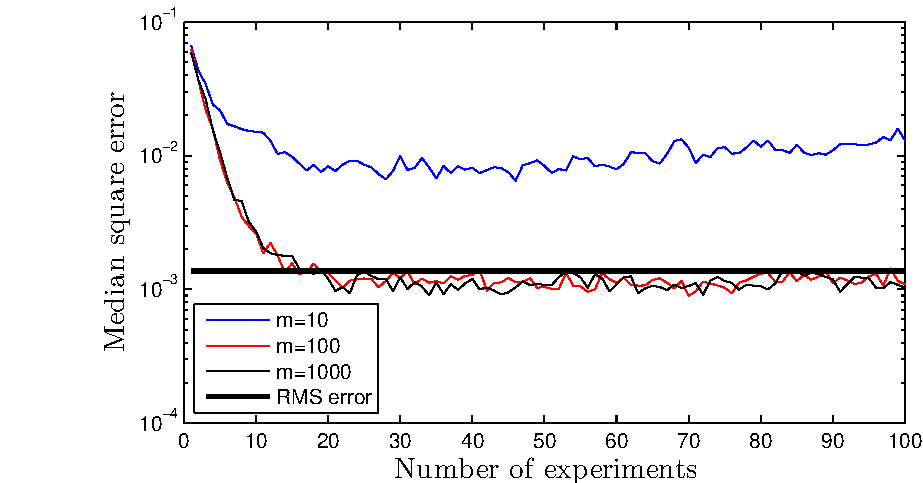
\includegraphics[width=0.99\columnwidth]{crej-diffusion3.pdf}
    }
    \caption{
        \label{fig:crej-diffusion}
        Rejection filtering with diffusion in the true model according to
        a normal random walk with standard deviation $\pi / 120$.  As expected, the error asymptotes to a value that is slightly less than the RMS error.
    }
\end{figure}

We design experiments $(x_-, t)$ using a heuristic that picks $x_-$ to be a random
vector sampled from the prior and $t=1/\sqrt{{\rm Tr}~ \Sigma}$ \cite{wiebe_efficient_2015}.
We use this heuristic here because it is known
to saturate the Bayesian Cramer--Rao bound for this problem and is
much faster than adaptively choosing $(t,x_-)$ to minimize the Bayes risk, which
we take to be the expected quadratic loss after performing an experiment given
the current prior.

The performance of \CRej~applied to this case is shown ~\fig{crej-diffusion}.
In particular, the median error incurred by \CRej~achieves the optimal
achievable error $(\pi / 120)^2$ with as few as $m = 100$ sampling attempts.
Thus, our \CRej~algorithm continues to be useful in the case of time-dependent
and other state-space models.  Although this demonstration is quite simple, it
is important to emphasize the miniscule memory requirements for this task
mean that this tracking problem can be solved using a small processor in
close proximity to the device in question.

%-----------------------------------------------------------------------------
\subsection{Handwriting Recognition}
%-----------------------------------------------------------------------------

A more involved example is handwriting recognition.  Our goal in this task is to use
Bayesian inference to classify an unknown digit taken from the MNIST repository~\cite{lecun1998mnist} in
one of two classes.  Here we consider two cases: $1$ vs $0$ and even vs odd.

We cast the problem in the language of Bayesian inference by assuming the likelihood
function
\begin{equation}
P(E|x;i,\sigma)\propto e^{-(x_i - E)^2/2\sigma^2}\label{eq:gausseq},
\end{equation}
which predicts the probability that a given pixel $i$ takes the value $E$,
given that the training image $x$ is the true model that it drew from.

We pick this likelihood function because if we imagine measuring every pixel in the image then the
posterior probability distribution, given a uniform initial distribution, will typically be sharply peaked around
the training vector that is closest to the observed vector of pixel intensities.
Indeed, taking the product over all pixels in an image produces the radial basis function
familiar to kernel learning \cite{scholkopf_learning_2001}.

\begin{figure}
\centering
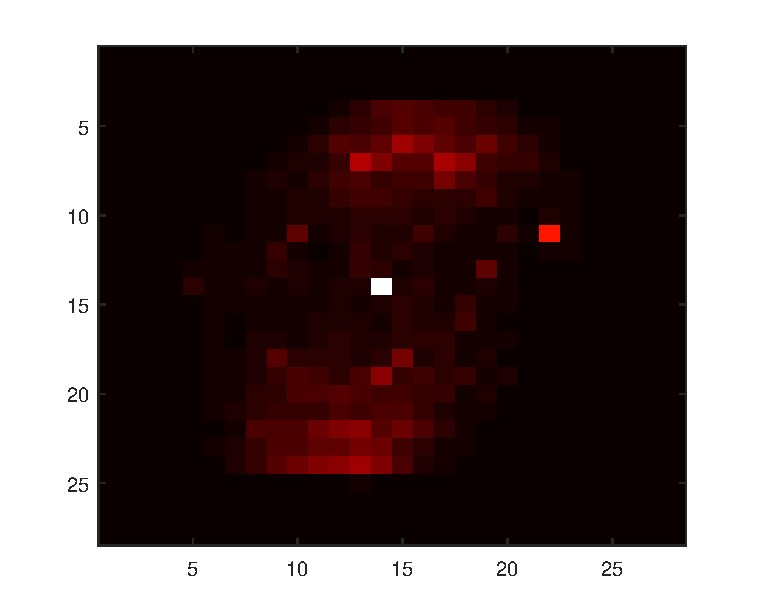
\includegraphics[width=0.49\columnwidth]{expHM.pdf}
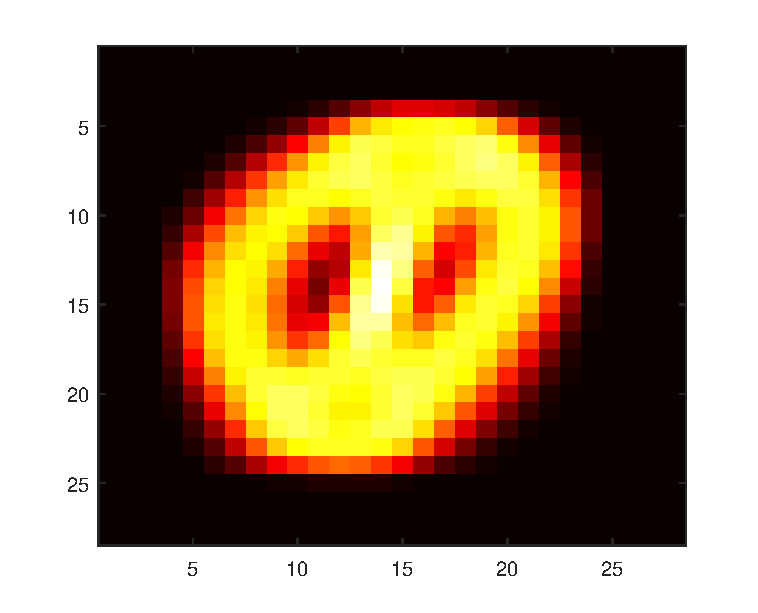
\includegraphics[width=0.49\columnwidth]{01HM.pdf}
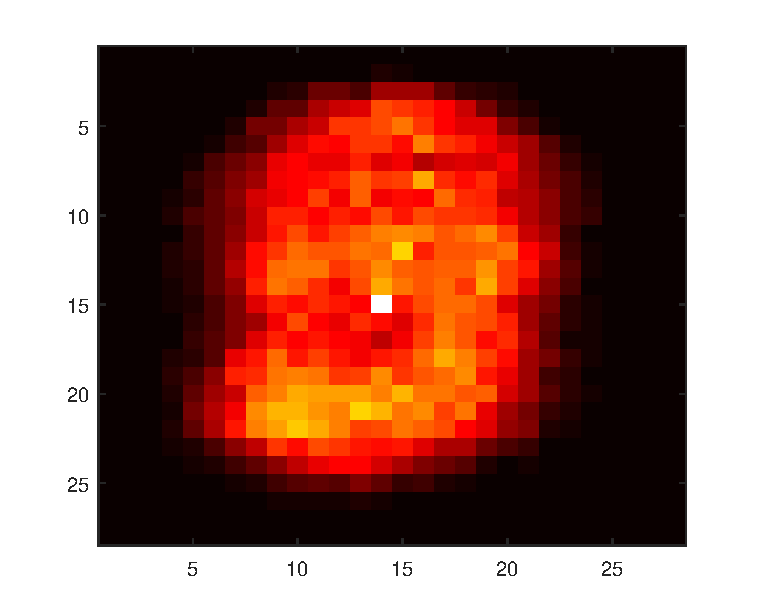
\includegraphics[width=0.49\columnwidth]{OEexpHM.pdf}
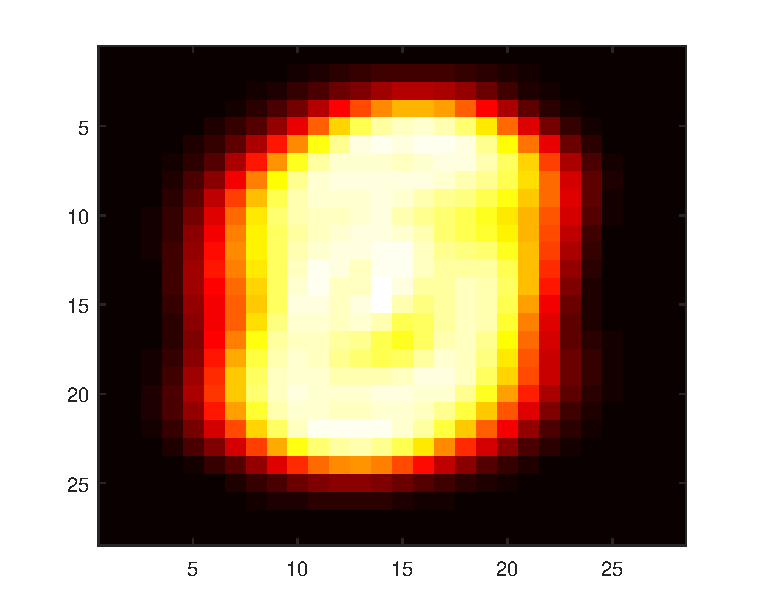
\includegraphics[width=0.49\columnwidth]{OEHM.pdf}
\caption{(top left) Heat map of frequency pixel is queried in zero vs one data set.  (top right) Heat map of variance of pixel data over data set.
Bottom plots are the corresponding plots for the odd/even digits.}\label{fig:HM}
\end{figure}

Unlike the previous experiment, we do not implement this in a memory--restricted
setting because of the size of the MNIST training set.
Our goal instead is to view the image classification problem through the lens of active learning.  In such
problems, it is assumed that the feature data is very expensive to compute.  This happens frequently
in search wherein features, such as page rank, can be expensive to compute on the fly.  It also can
occur in experimental sciences where each data point may take minutes or hours to either measure
or compute accurately.  In these cases it is vital to minimize the number of queries made to the training
data.  We will show that our Bayesian inference approach to this problem allows this to be solved using
far fewer queries than other methods, such as kNN, would require.  We also show that our method can
be used to \emph{extract} the relevant important features (i.e. pixels) from the data set.

We perform these experiments using an adaptive guess heuristic, similar to that employed in the frequency estimation example.
The heuristic works by choosing the pixel label, $i$, to query that has the largest variance of intensity
over the $m$ training vectors that compose the particle cloud.  We then pick $\sigma$ to be the standard
deviation of the intensity of that pixel.  This method has the advantage that once the set of particles
considered becomes small then the variance shrinks and allowing $\sigma$ to shrink proportionally dramatically
speeds up the inference process.  

\begin{figure}
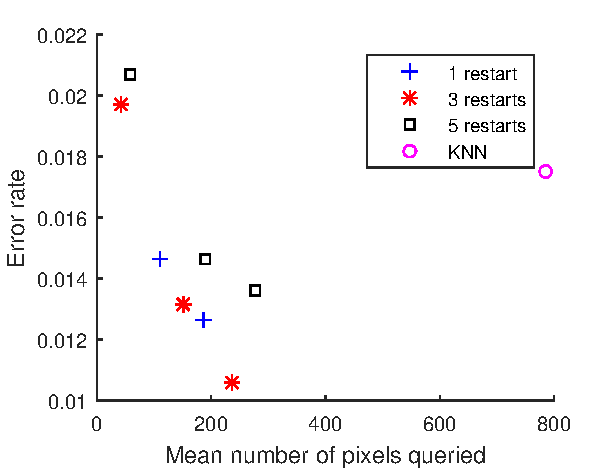
\includegraphics[width=\columnwidth]{ErrorPlot.pdf}
\caption{Classification errors for odd/even MNIST digits for rejection filtering with 784 maximum experiments distributed over 1,3,5 restarts and stopping condition $\mathcal{P}=0.1,0.01,0.001$.}\label{fig:errorplot}
\end{figure}

We repeat this process of querying pixels until the sample probability distribution has converged to a distribution that
assigns probability at most $\mathcal{P}$ to one of the two classes in the problem.  This process is restarted a total of
$1,3$ or $5$ times subject to the constraint that at most $784$ queries are made in the inference process (divided equally over each of the restarts).
The label assigned to the test vector is then the most frequently appearing label out of these tests.  This choice ensures that our method will at most
incurr the same cost as na\i ve kNN, but is pessimistic we do not allow the algorithm to store the results of prior queries which could reduce the 
complexity of the inference.

We make one further modification of the rejection filtering algorithm in order to fit it to this problem.  Since our classification problem has only two classes, we cannot directly apply the resampling step as described in~\alg{crej}.  Instead, we use a method similar to the bootstrap filter.  Specifically, when resampling we draw a number of particles from both
classes proportional to the sample frequency in the posterior distribution.  For each of these classes we then replicate the surviving particles until $95\%$ of the total population is replenished
by copies from the posterior cloud of samples.  The remaining $5\%$ are drawn uniformly from the training vectors with the corresponding class labels.

\fig{HM} illustrates the differences between maximum variance experiment design and the adaptive method we use in rejection filtering.  These differences
are perhaps most clearly seen in the problem of classifying one vs zero digits from MNIST.  Our adaptive approach most frequently queries the middle pixel, which is the 
highest variance feature over the training set.  This is unsurprising, but the interesting fact is that the second most frequently queried pixel is one that has relatively low variance
over the training set.  In contrast, many of the high-variance pixels near the maximum variance pixel are never queried despite the fact that they have large variance over the set.
This illustrates that they carry redundant information and can be removed from the training set.  Thus this adaptive learning algorithm can also be used to provide a type of model compression, similar to PCA.

The case for odd vs even is more complicated.  This is because the hand written examples have much less structure in them and so it is perhaps unsurprising that less dramatic compression is possible when examining that class. However, the data still reveals qualitatively that even here there is a disconnect between the variance of the features over the training set and their importance in classification.

We will now go beyond these qualitative discussions to quantitatively compare rejection filtering to kNN classification.  kNN is known to perform well for digit classification but it can be prohibitively slow for
large training sets (indexing strategies can be used to combat this problem~\cite{yu2001indexing}).  In order to make the comparison as fair as possible between the two, we compare kNN to rejection filtering by truncating the 
MNIST examples by removing pixels that have low variance over the training set.  This removes some of the advantage our method has by culling pixels near
the boundary of the image that contain very little signal  (see~\fig{HM}) and yet substantially contribute to the cost of kNN in an active learning setting.

Further optimizations can be used to improve the performance of kNN such as feature extraction~\cite{zhang2006svm,weinberger2008fast,min2009deep} or the use of 
deformation models~\cite{keysers2007deformation};
however we suspect that they will only serve to improve the performance of both methods. We leave investigation of the performance of rejection filtering under such optimization
for future work.

\fig{errorplot} shows that in certain parameter regimes, approximate Bayesian inference via rejection sampling can not only achieve higher classification accuracy on average for a smaller
number of queries to the test vector, but also can achieve $25\%$ less error even if these constraints are removed.  This result is somewhat surprising given that we chose our likelihood function to correspond to nearest neighbor classification if $\sigma$ is held constant.  However, we do not hold $\sigma$ constant in our inference but rather choose it adaptively as the experiment proceeds.  This fact changes the weight of the evidence provided by each pixel query and explains why it is possible for our algorithm to outperform kNN classification despite the apparent similarities between the two approaches.

%=============================================================================
\section{Conclusion}
\label{sec:conclusions}
%=============================================================================

We introduce a method, rejection filtering, that integrates
rejection sampling with particle filtering. Rejection filtering retains many of the benefits
of each, while using substantially less memory than conventional methods for Bayesian inference in typical use cases.
In particular, if a Gaussian resampling algorithm is used then our method only requires remembering a single sample at a time, making it ideal
for memory-constrained and active learning applications.
We further illustrate the viability of our rejection filtering approach through numerical experiments
involving tracking the time-dependent drift of an unknown frequency and also in handwriting recognition.

While our work has shown that rejection sampling can be a viable method for performing Bayesian inference, there are many
avenues for future work that remain open.  One such avenue involves investigating whether ideas borrowed from the particle
filter literature, such as the unscented transformation~\cite{van2000unscented} or genetic mutation-selection algorithms~\cite{del2012adaptive,del2000branching}, can be adapted to fit our setting.
  These improvements may help mitigate the information loss that necessarily occurs in the resampling step.  An even more exciting
application of these ideas may be to examine their application in online data acquisition in science and engineering.  Rejection
filtering provides the ability to perform adaptive experiments using embedded hardware, which may lead to a host of applications
within robotics and experimental physics that are impractical with existing technology.

%% END MATTER %%%%%%%%%%%%%%%%%%%%%%%%%%%%%%%%%%%%%%%%%%%%%%%%%%%%%%%%%%%%%%%%

\appendix

%=====================================================================
\subsubsection*{Acknowledgements}
%=====================================================================

%=====================================================================
\bibliographystyle{unsrt}
\bibliography{qsmc}
%=====================================================================


\clearpage
\onecolumn

% Copied from aistats2015.sty to disable setting running head.
\thispagestyle{empty}
  \hsize\textwidth
  \linewidth\hsize \toptitlebar {\centering
  {\Large\bf \thetitle:\\ Supplemental Material \par}}
 \bottomtitlebar \vskip 0.2in plus 1fil minus 0.1in

%=============================================================================
\section{Proofs of Theorems}
%=============================================================================

In this Appendix, we present proofs for the theorems presented in the main
body.

\begin{proofof}{\thm{crej}}
There are two parts to our claim in the theorem.  The first is that the rejection sampling algorithm is efficient given the theorem's assumptions
and the second is that it only requires $O({\rm dim}(x)^2 \log(1/\epsilon))$ memory to approximate the appropriate low--order moments of
 the posterior distribution.

For each of the $m$ steps in the algorithm the most costly operations are 
\begin{enumerate}
\item Sampling from $P$.
\item Sampling from the uniform distribution.
\item The calculation of $xx^T$.
\end{enumerate}
The first two of these are efficient by the assumptions of the theorem.  Although it may be tempting to claim that efficient algorithms are known
for sampling from the uniform distribution, the existence of such deterministic algorithms is unknown since it is not known whether the complexity
classes $\BPP$ and $\P$ coincide.  The remaining operation can be computed using $O({\rm dim}(x)^3)$ arithmetic operations, each of which can
be performed (to within bounded accuracy) efficiently on a Turing machine.  Therefore the cost of the inner loop is $O(m{\rm dim}(x)^3)$ which is efficient
if $m$ is taken to be a constant.

The remaining operations require at most $O({\rm dim}(x)^3)$ arithmetic operations and thus do not dominate the cost of the algorithm.  The main question remaining
is how large $m$ needs to be and how many bits of precision are required for the arithmetic.  Both the error in the mean and the elements of the covariance matrix scale as $O(1/\sqrt{N_a})$ where $N_a$ is the number of accepted samples that pass through the rejection filter.  Thus if both are to be computed within error $\epsilon$ then $N_a \in O(1/\epsilon^2)$.  However, in order to get a sample accepted we see from the Markov inequality and the definition of the exponential distribution that $m$ must scale like $m\in O(1/P_{\rm success} \epsilon^2)$.  We then see from~\cor{badalgorithm} that $P_{\rm success} \in \Omega(\min_x P(E|x)/\kappa_E)$, which we assume is at most polynomially small.  Ergo the sampling process is efficient given these assumptions and the fact that $\epsilon$ is taken to be a constant for the purposes of defining efficiency.

The dominant requirements for memory arise from the need to store $\Sigma$, $\mu\mu^T$ and $xx^T$.  There are at most $O({\rm dim}(x)^2)$ elements in those matrices and so if each is to be stored within error $\epsilon$ then at least $O({\rm dim}(x)^2\log(1/\epsilon))$ bits are required.  Note that the incremental formulas used in the algorithm are not very numerically stable and need $2N$-bit registers to provide an $N$-bit answer.  This necessitates doubling the bits of precision, but does not change the asymptotic scaling of the algorithm.  Similarly, the $m\in O(1/\epsilon^2)$ repetitions of the algorithm also does not change the asymptotic scaling of the memory because $\log(1/\epsilon^3) \in O(\log(1/\epsilon))$.

What does change the scaling is the truncation error incurred in the matrix multiplication.  The computation of a row or column of $xx^T$, for example, involves ${\rm dim}(x)$ multiplications and additions.  Thus if each such calculation were computed to to within error $\epsilon$, the total error is at most by the triangle inequality ${\rm dim}(x) \epsilon$.  Therefore in order to ensure a total error of $\epsilon$ in each component of the matrix we need to perform the arithmetic using $O(\log({\rm dim}(x)/\epsilon))$ bits of precision.  The result then follows.
\end{proofof}

\begin{proofof}{\lem{errprop}}
Using the definition of $\tilde{P}(x)$ and Bayes' rule it is easy to see that the error in the posterior mean is
\begin{align}
\Biggr| \int_V \frac{P(E|x)P(x)x}{\langle P(E|x),P(x) \rangle}\left( 1 - \frac{1}{1+\frac{\langle P(E|x),\Delta(x)\rangle }{\langle P(E|x),P(x) \rangle}}\right) - \frac{P(E|x) \Delta(x)x}{\langle P(E|x),P(x)\rangle}\left(\frac{1}{1+\frac{\langle P(E|x),\Delta(x)\rangle }{\langle P(E|x),P(x) \rangle}} \right)\mathrm{d}x \Biggr|.\label{eq:intbd}
\end{align}
Using the fact that $|1-1/(1-y)| \le 2|y|$ for all $y\in [-1/2,1/2]$ it follows from the assumptions of the theorem and the triangle inequality that~\eq{intbd} is bounded above by
\begin{align}
 \int_V \frac{2P(E|x)P(x)\|x\| |\langle P(E|x),\Delta(x) \rangle|}{\langle P(E|x),P(x) \rangle^2}\mathrm{d}x+ \int_V\frac{2P(E|x) |\Delta(x)|\|x\|}{\langle P(E|x),P(x)\rangle}\mathrm{d}x.\label{eq:intbd2}
\end{align}
Now using the fact that $\|x\|\le \|x_{\max}\|$ and the definition of the inner product, we find that~\eq{intbd2} is bounded above by
\begin{equation}
\frac{2 (|\langle P(E|x),\Delta(x) \rangle| + \langle P(E|x), |\Delta(x)| \rangle))\|x_{\max}\|}{\langle P(E|x),P(x)\rangle}.
\end{equation}
The  result then follows from a final application of the triangle inequality.

The analogous proof for the error in the posterior expectation of $xx^T$ follows using the exact same argument after replacing the Euclidean norm with the induced $2$--norm for matrices.  Since both norms satisfy the triangle inequality, the proof follows using exactly the same steps after observing that $\|xx^T\|\le \|x_{\max}\|^2$ for all $x\in V$.
\end{proofof}

\begin{proofof}{\thm{meanCov}}
\lem{errprop} provides an upper bound on the error in the mean of the posterior distribution that propagates from errors in the components of our prior distribution.  We then have that if we sample from this distribution then the sample standard deviation of each of the $N$ components of $x$ is $O(\sigma_{\max}/\sqrt{m})$.  Thus the sample standard deviation of $\sum_{i=1}^N (x_i-\tilde{\mu}_i)^2$ is at most $O(\sqrt{N}\sigma_{\max}/\sqrt{m})$.  The triangle inequality shows that the sampling error and the error that propagates from having an incorrect prior are at most additive. 

 The calculation for the error in the estimate of the covariance matrix is similar.  First, note that $1/(m-1)= 1/m +O(1/m^2)$ so we can asymptotically ignore $m/(m-1)$.  Let $\mu = \int_V P(x|E) x\mathrm{d}x +\epsilon v$, where $|v|=1$.  We then have from our error bounds on the estimate of the posterior mean that
\begin{eqnarray}
\| \mu\mu^T - \int_V P(x|E) x\mathrm{d}x \int_V P(x|E) x^T\mathrm{d}x \|&\le& \epsilon \left\|\int_V P(x|E) x\mathrm{d}x v^T\right\|+\epsilon\left\|v\int_V  P(x|E) x^T\mathrm{d}x\right\| + \epsilon^2.\nonumber\\
&\in&  O\left(\left[\frac{\sqrt{N}}{\sqrt{m}} +\frac{\langle P(E|x), |\Delta(x)|\rangle}{\langle P(E|x),P(x)\rangle}\right]\|x_{\max}\|^2\right).
\end{eqnarray}

Now let us focus on bounding the error in our calculation of $\int_V P(E|x) xx^T \mathrm{d}x$. Using the triangle inequality, the error in the estimate of the expectation value of $x x^T$ is, to within error $O(1/m^{3/2})$, at most
\begin{equation}
\Biggr\|\frac{1}{m} \sum_{j=1}^m x_j x_j^T - \int_V \tilde{P}(x|E) x x^T\mathrm{d}x\Biggr\|+\Biggr\| \int_V \tilde{P}(x|E) x x^T\mathrm{d}x-\int_V {P}(x|E) x x^T\mathrm{d}x\Biggr\|.\label{eq:xxT}
\end{equation}
The first term in \eq{xxT} can be bounded by bounding the sample error in each of the components of the matrix.  For any component $[xx^T]_{k,\ell}$ the Monte--Carlo error in its estimate is
\begin{equation}
O\left(\frac{\sigma({[x]_k[x]_\ell})}{\sqrt{m}}\right)\in O\left(\frac{\|x_{\max}\|^2}{\sqrt{m}}\right).
\end{equation}
The $2$--Norm of an $N\times N$ matrix is at most $N$ times its max--norm, which means that
\begin{equation}
\Biggr\|\frac{1}{m} \sum_{j=1}^m x_j x_j^T - \int_V \tilde{P}(x|E) x x^T\mathrm{d}x\Biggr\|\in O\left(\frac{N\|x_{\max}\|^2}{\sqrt{m}}\right).\label{eq:xxTMC}
\end{equation}
The theorem then follows from inserting~\eq{xxTMC} into~\eq{xxT} and applying~\lem{errprop}.
\end{proofof}

%=============================================================================
\section{Batched Updating}
\label{app:batched-updates}
%=============================================================================

Although we focused in the main body on memory restricted applications, it is also possible to exploit the fact that the
rejection sampling procedure is inherently parallelizable.
This comes at the price of increasing the overall
memory usage. Here, we describe a batched form of our algorithm, assuming a model in which samples are sent by a server to individual processing nodes and the accepted samples are then returned to the server.

\begin{algorithm}
    \caption{Batched update for \CRej}
    \label{alg:batchcrej}
    \begin{algorithmic}
        \Require Prior distribution $\pi:\mathbb{R}^D \mapsto [0,1]$, array of evidence $\vec{E}$, number of attempts $m$, a constant $0<\kappa_E\le 1$, a recovery factor $r \ge 0$, the prior mean $\mu$ and the covariance matrix $\Sigma$.
%        and a mapping $\operatorname{F}$ between $(\mu,\sigma^2)$ to a family of probability distributions that has mean $\mu$ and covariance matrix $\Sigma$. Typically $F$ will yield a Gaussian distribution but other possibilities exist.
        \Ensure  The mean and coviariance matrix of updated distribution $\mu$,$\Sigma$ and $N_a$ which is the number of samples accepted.
        \Function{BatchUpdate}{$\vec{E}$, $m$, $\kappa_E$, $\mu$, $\Sigma$, $r$, $N_{\rm batch}$}
  \State{$(M,S,N_a) \gets 0$}
          \For{{\bf each} $i \in 1 \to N_{\rm batch}$}
  \State Pass $\vec{E},m,\kappa_E, \mu,\Sigma,r$ to processing node $i$.
  \State Set local variables $(\mu^{i}, \Sigma^{i},N_a^{i})\gets \Call{RFUpdate}{\vec{E},m,\kappa_E,\mu,\Sigma,r}$.
  \If{$N_a^i >0$}
  \State $M^i \gets \mu^i N_a^i$
  \State $S^i \gets (N_a^i-1)\Sigma +N_a^i\mu\mu^T$ 
  \State Pass $N_a^i$, $M^i$ and $S^i$ back to the server.       
  \Else \State Pass $(0,0,0)$ back to the server.
  \EndIf
  \EndFor
    \If{$\sum_i N_a^i > 0$}
     \State $\mu\gets \sum_i M^{i}/\sum_i N_a^i $
     \State $\Sigma \gets \frac{1}{\sum_i N_a^i -1}\left(\sum_i S^i - \sum_i N_a^i \mu\mu^T \right)$
  \State\Return $(\mu,\Sigma,N_a)$
   \Else
  \State\Return $(\mu, (1+r)\Sigma),N_a)$

   \EndIf
          
        \EndFunction
    \end{algorithmic}
\end{algorithm}



\end{document}